% Created 2016-09-17 Sat 13:31
\documentclass[a4paper]{article}
\usepackage[utf8]{inputenc}
\usepackage[T1]{fontenc}
\usepackage{fixltx2e}
\usepackage{graphicx}
\usepackage{grffile}
\usepackage{longtable}
\usepackage{wrapfig}
\usepackage{rotating}
\usepackage[normalem]{ulem}
\usepackage{amsmath}
\usepackage{textcomp}
\usepackage{amssymb}
\usepackage{capt-of}
\usepackage[hyperref,x11names]{xcolor}
\usepackage[colorlinks=true,urlcolor=SteelBlue4,linkcolor=Firebrick4]{hyperref}
% --------------INTEGRATION CODE JAVA----------
\usepackage{listings}
\lstset{
language=Java,
basicstyle=\normalsize, % ou ça==> basicstyle=\scriptsize,
upquote=true,
aboveskip={1.5\baselineskip},
columns=fullflexible,
showstringspaces=false,
extendedchars=true,
breaklines=true,
showtabs=false,
showspaces=false,
showstringspaces=false,
identifierstyle=\ttfamily,
keywordstyle=\color[rgb]{0,0,1},
commentstyle=\color[rgb]{0.133,0.545,0.133},
stringstyle=\color[rgb]{0.627,0.126,0.941},
}

\author{Willian Ver Valen Paiva \and Alan Guitard}
\date{\today}
\title{Rapport TP2}
\hypersetup{
 pdfauthor={Willian Ver Valen Paiva},
 pdftitle={Rapport TP2},
 pdfkeywords={},
 pdfsubject={},
 pdfcreator={Emacs 25.1.50.1 (Org mode 8.3.5)}, 
 pdflang={fr}}
\begin{document}

\maketitle

\tableofcontents

\label{sec:orgheadline14}
\section{the API}
\label{sec:orgheadline8}
\subsection{org.apache.hadoop.conf.Configuration}
\begin{lstlisting}
@InterfaceAudience.Public
@InterfaceStability.Stable
public class Configuration
extends Object
implements Iterable<Map.Entry<String,String>>, Writable
\end{lstlisting}
\label{sec:orgheadline1}
Cette classe est chargé de fournir un accès à la configuration des paramètres depuis le répertoire de configuration.

\subsection{org.apache.hadoop.conf.Configured}
\label{sec:orgheadline2}

\begin{lstlisting}
@InterfaceAudience.Public
@InterfaceStability.Stable
public class Configured
extends Object
implements Configurable
\end{lstlisting}
Les objets pouvant être configurés par un objet de type \verb?Configuration? étendront cette classe.
\subsection{org.apache.hadoop.fs.FileSystem}
\label{sec:orgheadline3}

\begin{lstlisting}
@InterfaceAudience.Public
@InterfaceStability.Stable
public abstract class FileSystem
extends Configured
implements Closeable
\end{lstlisting}
Cette classe est utilisé pour accéder un fichier distribué d'Hadoop.
\subsection{org.apache.hadoop.fs.Path}
\label{sec:orgheadline4}
\begin{lstlisting}
@Stringable
@InterfaceAudience.Public
@InterfaceStability.Stable
public class Path
extends Object
implements Comparable
\end{lstlisting}
Cette classe contient le nom et le chemin d'un fichier de classe \verb?FileSystem?.
\subsection{org.apache.hadoop.io.IOUtils}
\label{sec:orgheadline5}
\begin{lstlisting}
@InterfaceAudience.Public
@InterfaceStability.Evolving
public class IOUtils
extends Object
\end{lstlisting}
Cette classe est une boîte à outils qui contient des fonctions d'entrée/sortie.
\subsection{org.apache.hadoop.util.Tool}
\label{sec:orgheadline6}
\begin{lstlisting}
@InterfaceAudience.Public
@InterfaceStability.Stable
public interface Tool
extends Configurable
\end{lstlisting}
Cette interface est en charge des options en ligne de commande génériques.
\subsection{org.apache.hadoop.util.ToolRunner}
\label{sec:orgheadline7}
\begin{lstlisting}
@InterfaceAudience.Public
@InterfaceStability.Stable
public class ToolRunner
extends Object
\end{lstlisting}
Cette classe implémente l'interface \verb?Tool? et lance donc les lignes de commandes qu'on lui passe en argument dans sa méthode run().

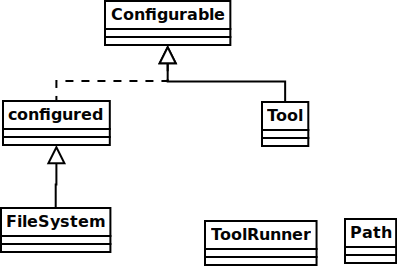
\includegraphics[width=.9\linewidth]{diagram.png}

\section{Deux premiers programmes d'exercices}
\label{sec:orgheadline11}
Comme l'implémentation de ces programmes ont été donnés en classe, notre solution sera donc plutôt similaire.
Nous allons donc expliquer comment ces programmes fonctionne pas à pas.
\subsection{La base}
\label{sec:orgheadline9}
La première étape est de créer un objet implémentant \verb?Tool? qui implémentera donc la méthode de run(), laquelle sera appelée en conjonction avec la méthode run() de \verb?ToolRunner?.
\subsection{La méthode run()}
\label{sec:orgheadline10}
C'est dans cette méthode que tout le programme se situe.
Voici décrit ci-après les étapes suivies pour accomplir la fonctionnalité du premier programme:
\begin{enumerate}
\item Créer un objet URI avec le chemin de sortie (fichier sur le HDFS).
\item Normaliser l'URI, ce qui signifie supprimer les points ou double-points du chemin, par exemple.
\item Créer l'objet de classe \verb?Path? à partir de l'URI normalisé.
\item Créer un object de classe \verb?Configuration? et y charger l'actuel configuration via la fonction \verb?getConf()?.
\item Créer un object de classe \verb?FileSystem? spécifiant le chemin, la configuration et l'utilisateur.
\item Créer les objets utiles à l'écriture, \verb?OutputStream?, sur le fichier nouvellement créé.
\item Créer les objets utiles à la lecture, \verb?InputStream?, sur le fichier local.
\item Copier les bytes de l'\verb?InputStream? vers \verb?OutputStream?.
\item Fermer les flux.
\end{enumerate}

Pour le second programme, les étapes sont plutôt, à l'exception de l'étape 7 et de celle qui suivent:
\begin{enumerate}
\setcounter{enumi}{7}
\item Créer une boucle pour lire chaque fichier.
\item Créer les objets utiles à la lecture, \verb?InputStream?, sur le fichier local courant.
\item Copier les bytes de l'\verb?InputStream? vers \verb?OutputStream?.
\item Fermer les flux de lecture.
\end{enumerate}
et, après la fin de ces actions sur tout les fichiers, fermer le flux d'écriture.

\section{Troisième exercice: Génération de mots}
\label{sec:orgheadline12}
L'implémentation de ce dernier exercice ne diffère pas énormément des deux précédents.
Pour accomplir l'objectif, trois fonctions ont été implémentées:

\begin{lstlisting}
public static char getRandom(char[] array) {
    int rnd = new Random().nextInt(array.length);
    return array[rnd];
}

public static String randomSyllable(){
    char[] alphabet = "abcdefghijklmnopqrstuvwxyz".toCharArray();
    return  new StringBuilder().append(getRandom(alphabet)).append(getRandom(alphabet)).toString();
}

public static String randomWord(int size){
    String exampleString = "";
    for(int i=0 ; i < size; i++){
        exampleString += randomSyllable();
    }
    return exampleString + " ";
 }
\end{lstlisting}

Ensuite, le même code que le précédent exercice en changeant la boucle pour itérer un nombre de fois définis en argument.
La façon dont le flux de lecture a été crée est aussi modifié:
\begin{lstlisting}
InputStream is = new ByteArrayInputStream(randomWord(10).getBytes(StandardCharsets.UTF_8));
\end{lstlisting}

Cette modification est nécessaire pour lire les bytes non plus à partir d'un fichier mais d'une chaîne de caractères.


\section{Exercice 7: Temps d’exécution}
\label{sec:orgheadline13}
Dans cet exercice, nous pouvons la différence de temps d'exécution entre ce programme et le script écrit dans l'exercice 4. 
La version écrite en Java est bien plus rapide. 
Ceci s'explique par le fait que la version script ouvre et ferme un descripteur de fichier sur chaque fichier, ce qui est une opération coûteuse en temps. En l'occurence, sur la version de Java, le descripteur de fichier s'ouvre sur le HDFS jusqu'à ce que tout les fichiers soit concaténés à l'intérieur, puis se ferme, ce qui réduit considérablement le nombre d'opérations dans la version Java.
\end{document}